\label{pd-datenmodell}
\section{Datenmodell}
Die Domain Logik ist weitestgehend im \gls{Backend} implementiert, welches die Daten über eine \gls{REST}-Schnittstelle zur Verfügung stellt.
Die über die Schnittstelle zur Verfügung gestellten Informationen sind also Ausgangspunkt für die von uns verwendbaren Domain Klassen.
Es waren kleinere Anpassungen nötig, etwa um den neuen Validationsmechanismus zu unterstützen.
Da die empfangenen Daten fast ausschliesslich als Repräsentation von Informationen dienen und keine eigene Logik implementieren, wurden sie als \glslink{DTO}{DTOs} umgesetzt.\newline
Das folgende Datenmodell repräsentiert die \glslink{DTO}{Datentransferobjekte} und ist nicht als semantisches Modell zu verstehen.\newline
\begin{figure}[H]
 	\centering
 	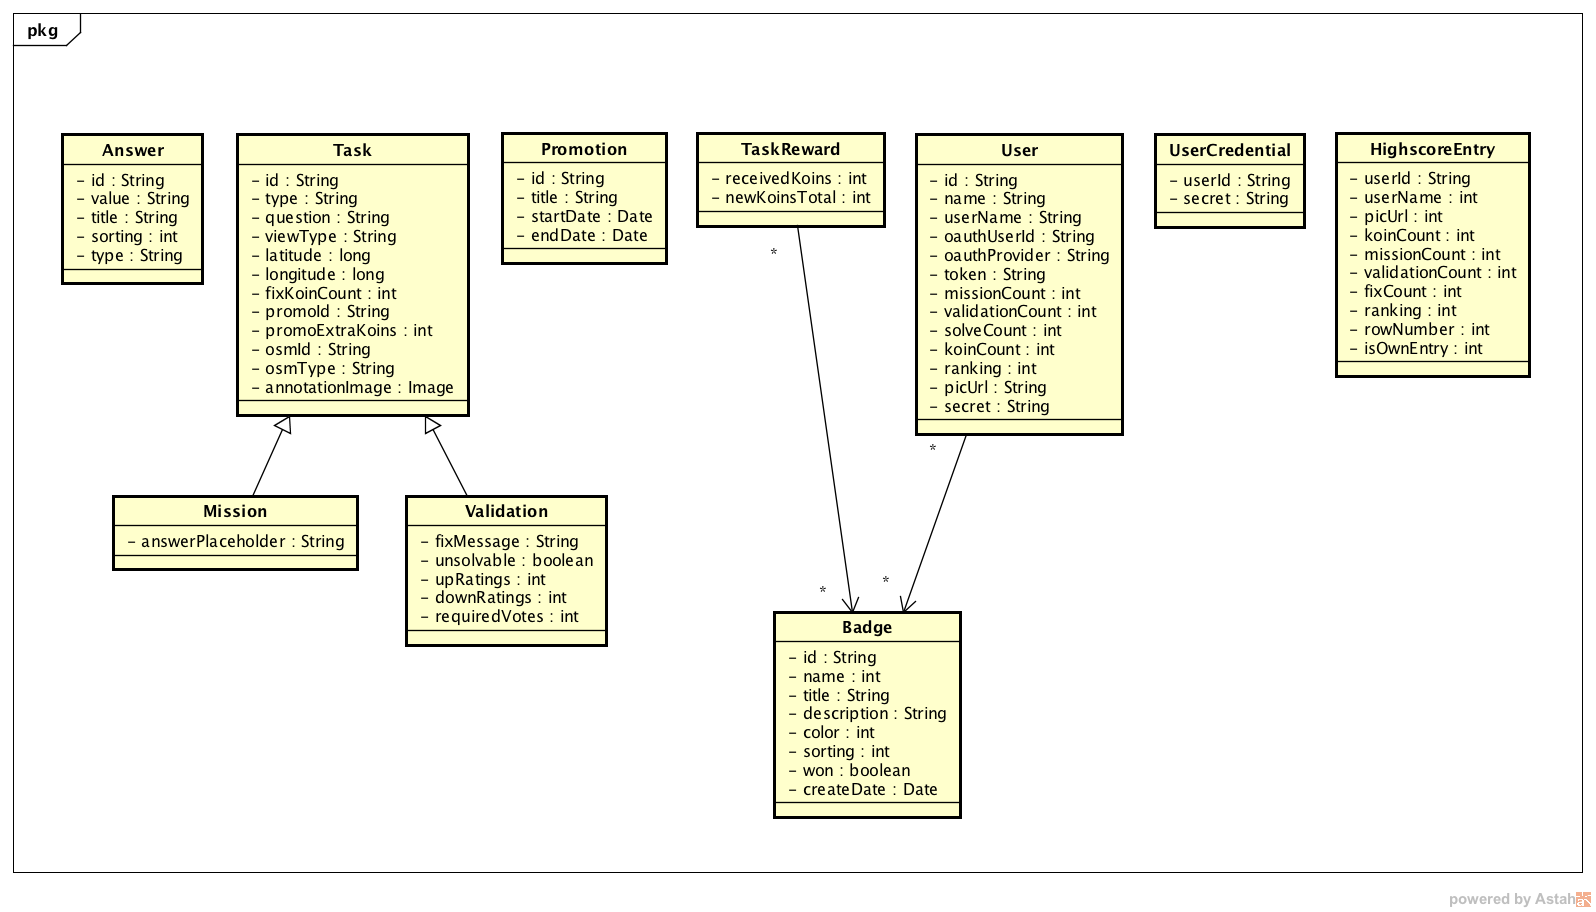
\includegraphics[width=\textwidth]{images/projektdokumentation/Datenmodell.png}
 	\caption{Modellierung der DTOs}
 	\label{image-data-model}
\end{figure}
